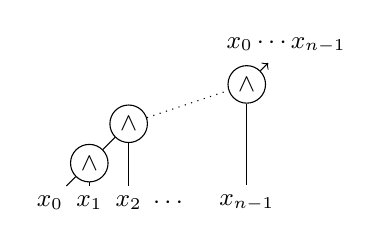
\begin{tikzpicture}[
    gate/.style={circle, draw, inner sep=2pt},
    every node/.style={font=\small}
]

% Inputs
\node (x0) at (-0.5,0) {$x_0$};
\node (x1) at (0,0) {$x_1$};
\node (x2) at (0.5,0) {$x_2$};
\node at (1,0) {$\cdots$};
\node (xn) at (2,0) {$x_{n-1}$};

% AND nodes
\node[gate] (a1) at (0,0.5) {$\wedge$};
\node[gate] (a2) at (0.5,1) {$\wedge$};
\node[gate] (ak) at (2,1.5) {$\wedge$};

% Output
\node (out) at (2.5,2) {$x_0\cdots x_{n-1}$};

% Edges
\draw (x0) -- (a1);
\draw (x1) -- (a1);
\draw (x2) -- (a2);

\draw (a1) -- (a2);
\draw[dotted] (a2) -- (ak);

\draw (xn) -- (ak);

\draw[->] (ak) -- (out);

\end{tikzpicture}
